\documentclass[a4j,10pt]{jsarticle}
\usepackage{layout,url,resume}
\usepackage[dvipdfmx]{graphicx}
\pagestyle{empty}

\begin{document}
%\layout

\title{スマートフォンのブラウザで視聴中のWebページ・動画の視聴位置を保存・復旧するしおりアプリ}

% 和文著者名
\author{
    Arch B3 新真虎(masatora) \thanks{慶應義塾大学環境情報学部}
    \and
    Adviser: 松谷健史(macchan) \thanks{慶應義塾大学大学院 政策・メディアメディア研究科特任講師}
}

% 和文概要
\begin{abstract}
ホセ・アブレイユ
\end{abstract}

\maketitle
\thispagestyle{empty}

\section{背景}
うんこち

%---------------------------------------------

\section{目的}


\section{アプローチ}

\section{実装}

\section{評価}

\section{結論}

\bibliographystyle{junsrt}
\bibliography{resume}

\section{記法参考}
\subsection{hoge}
小見出し付きの文章.

\begin{enumerate}
\item 番号付き箇条書き 
\item 番号付き箇条書き
\end{enumerate}

\begin{itemize}
\item 箇条書き
\item 箇条書き
\end{itemize}

\subsection{hoge}
画像を図\ref{sample}に示す。

\begin{figure}[htbp]
    \begin{center}
        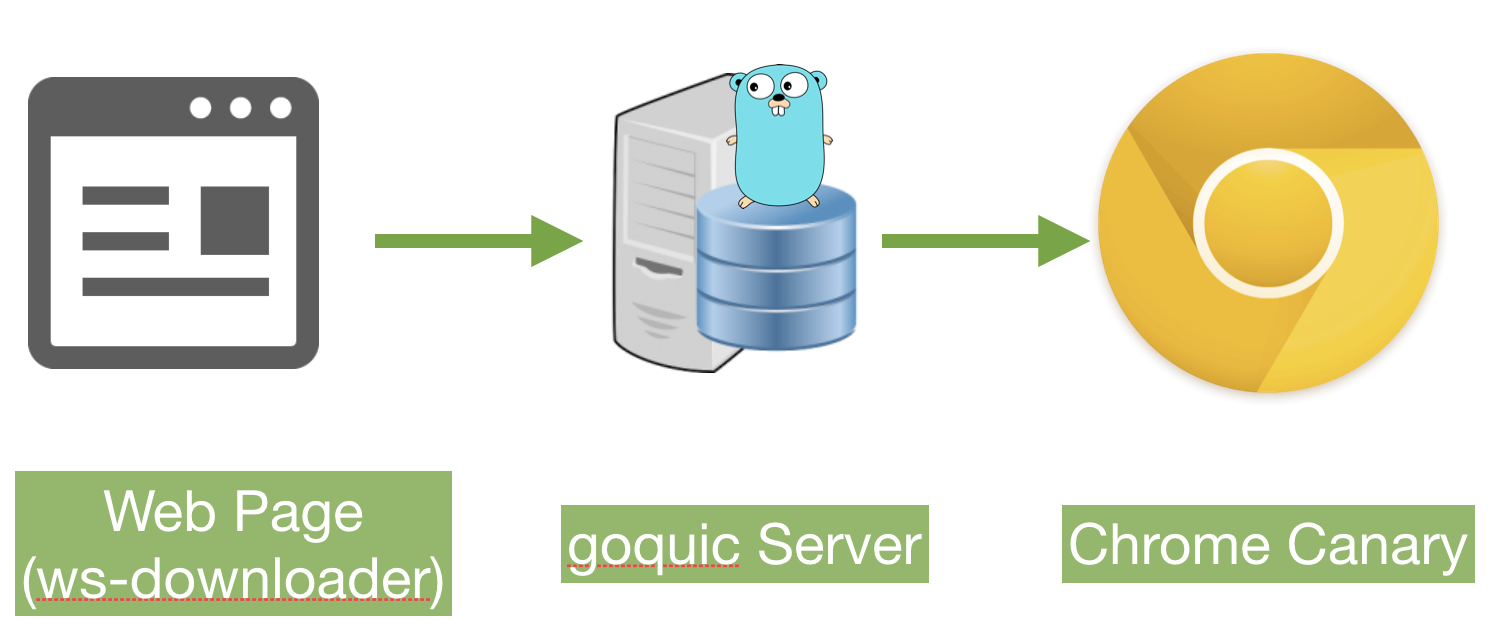
\includegraphics[width=6cm]{figure1.png}
        \caption{画像の例}
        \label{sample}
    \end{center}
\end{figure}
 
\subsection{fuga}
fugafuga

\end{document}
% end of file
